

\documentclass[reprint,english,notitlepage]{revtex4-1}  % defines the basic parameters of the document

% if you want a single-column, remove reprint

% allows special characters (including æøå)
\usepackage[utf8]{inputenc}
\usepackage[english]{babel}


\newcommand*{\QEDA}{\hfill\ensuremath{\blacksquare}}
\usepackage{amsmath, amssymb}

%% note that you may need to download some of these packages manually, it depends on your setup.
%% I recommend downloading TeXMaker, because it includes a large library of the most common packages.

\usepackage{physics,amssymb}  % mathematical symbols (physics imports amsmath)
\usepackage{graphicx}         % include graphics such as plots
\usepackage{xcolor}           % set colors
\usepackage{hyperref}    
\usepackage{filecontents}
% automagic cross-referencing (this is GODLIKE)
\usepackage{tikz}             % draw figures manually
\usepackage{listings}         % display code
\usepackage{subfigure}        % imports a lot of cool and useful figure commands



% defines the color of hyperref objects
% Blending two colors:  blue!80!black  =  80% blue and 20% black
\hypersetup{ % this is just my personal choice, feel free to change things
    colorlinks,
    linkcolor={red!50!black},
    citecolor={blue!50!black},
    urlcolor={blue!80!black}}

%% Defines the style of the programming listing
%% This is actually my personal template, go ahead and change stuff if you want
\lstset{ %
	inputpath=,
	backgroundcolor=\color{white!88!black},
	basicstyle={\ttfamily\scriptsize},
	commentstyle=\color{magenta},
	language=Python,
	morekeywords={True,False},
	tabsize=4,
	stringstyle=\color{green!55!black},
	frame=single,
	keywordstyle=\color{blue},
	showstringspaces=false,
	columns=fullflexible,
	keepspaces=true}

%% USEFUL LINKS:
%%
%%   UiO LaTeX guides:        https://www.mn.uio.no/ifi/tjenester/it/hjelp/latex/ 
%%   mathematics:             https://en.wikibooks.org/wiki/LaTeX/Mathematics

%%   PHYSICS !                https://mirror.hmc.edu/ctan/macros/latex/contrib/physics/physics.pdf

%%   the basics of Tikz:       https://en.wikibooks.org/wiki/LaTeX/PGF/TikZ
%%   all the colors!:          https://en.wikibooks.org/wiki/LaTeX/Colors
%%   how to draw tables:       https://en.wikibooks.org/wiki/LaTeX/Tables
%%   code listing styles:      https://en.wikibooks.org/wiki/LaTeX/Source_Code_Listings
%%   \includegraphics          https://en.wikibooks.org/wiki/LaTeX/Importing_Graphics
%%   learn more about figures  https://en.wikibooks.org/wiki/LaTeX/Floats,_Figures_and_Captions
%%   automagic bibliography:   https://en.wikibooks.org/wiki/LaTeX/Bibliography_Management  (this one is kinda difficult the first time)
%%   REVTeX Guide:             http://www.physics.csbsju.edu/370/papers/Journal_Style_Manuals/auguide4-1.pdf
%%
%%   (this document is of class "revtex4-1", the REVTeX Guide explains how the class works)


%% CREATING THE .pdf FILE USING LINUX IN THE TERMINAL
%% 
%% [terminal]$ pdflatex template.tex
%%
%% Run the command twice, always.
%% If you want to use \footnote, you need to run these commands (IN THIS SPECIFIC ORDER)
%% 
%% [terminal]$ pdflatex template.tex
%% [terminal]$ bibtex template
%% [terminal]$ pdflatex template.tex
%% [terminal]$ pdflatex template.tex
%%
%% Don't ask me why, I don't know.
\begin{document}
\title{FYS-STK 4155 Project 3 
Additional Exercise: \\
Bias-Variance Tradeoff Analysis in the Context of Regression} \\ 
\large{}
\author{Lasse Totland, Domantas Sakalys, Synne Mo Sandnes, Semya A. Tønnessen}
\date{\today}      % self-explanatory
\noaffiliation                            % ignore this
\begin{abstract} 
In this bonus project, we perform an analysis of the bias-variance tradeoff in the context of regression. We analyze the bias-variance and Mean Square Error (MSE) for linear regression using Ordinary Least Squares (OLS) and Ridge, then deep learning using a Multi-Layer Perceptron (MLP) model and finally we look at ensemble methods using decision trees and random forests. All methods are tested using the Franke function as our data set. Overall we find that the Ridge method produces results with both low bias and variance while saving computational time. The overall MSE is consistently quite low for this model. Random forests also produce good results, achieving a lower bias in a shorter amount of time than Ridge. However, this model requires more computational time. 
\end{abstract}

\maketitle % creates the title, author, date & abstract

\section{Introduction}
In this exercise, the aim is to perform an analysis of the bias-variance tradeoff in the context of regression. We use three of the methods previously discussed in the course: Linear Regression using the Ordinary Least Square (OLS) method and Ridge regression~\cite{proj1}, then deep learning using a Feed Forward Neural Network (FFNN)~\cite{proj2}, and finally Ensemble methods using decision trees and random forests~\cite{proj3}. 
For an overview of these algorithms, we refer to our previous projects from this course, cited in the reference section. 
\vspace{3mm}
\\ 
For any supervised machine learning algorithm, we can decompose the error into bias and variance. Bias indicates the difference between the predictions of the model and the true values, while the variance deals with the spread of the data. A model with high bias oversimplifies the prediction and will underfit the data. Meanwhile, a model with high variance fit the training data closely, but will be unable to fit new data that it has not previously trained on, and so the data will be overfitted. 
Finding the right balance between both components as we attempt to minimize them is called the bias-variance tradeoff~\cite{morthen}. 
\vspace{3mm}
\\ 
When choosing a model for a regression problem, it is important to consider both the bias and variance.
Simple models, such as linear and logistic regression models, generally have a high bias and a low variance. More complex models, such as random forests, generally have a lower bias but higher variance. 
\vspace{3mm}
\\ 
We will study the bias-variance as a function of the complexity of the model using the Franke function as our data set. 
In section~\ref{sec: method} we introduce bias-variance in further detail. Our results and a discussion of these are presented in section~\ref{sec: results}, before we go over the conclusion and final outlook in section~\ref{sec: conclusion}. 




\section{Method}\label{sec: method}
\subsection*{Bias-Variance}
The aim of supervised machine learning problems is to find a mathematical representation $f$ which can explain the relationship between input predictors $\boldsymbol{x}$ and an observed outcome $\boldsymbol{y}$
\begin{align}
    \boldsymbol{y} = f(\boldsymbol{x}) + \epsilon, 
\end{align}
where $\epsilon$ is some noise in the data. The algorithm learns from a training data set and iteratively makes predictions on the training data, in a process that can be thought of as learning. The learning stops when the algorithm achieves an acceptable level of performance. 
\vspace{3mm}
\\
The bias-variance is an estimate of how well an approximation performs, visualized by studying the complexity of the model. In order to find a measure of the expected error in a function, we want to minimize the error in the model when predicting the outcome from the predictors. Such an error is usually a measure of distance between the predicted outcome and the observed outcome, for all observations. For this aim, we can use the MSE, 
\begin{align}\label{eq: MSE}
    MSE\left(\boldsymbol{y},\boldsymbol{\tilde{y}}\right) = \frac{1}{n}\sum\limits_{i=0}^{n-1}{\left(y_i - \tilde{y}_i\right)}^2
\end{align}
The error can be decomposed into the sum of three quantities, 
\begin{align}
    \mathbb{E}[(\boldsymbol{y} - \boldsymbol{\tilde{y}})^2] 
    &= (\text{Bias}[\tilde{y}])^2 
        + \text{Var}[\tilde{f}] 
        + \sigma^2, 
\end{align}
The bias of the model $\boldsymbol{\tilde{y}}$ compared to the continuous function $\boldsymbol{f}$ that we wish to obtain is given by 
\begin{align}
    (\text{Bias}[\tilde{y}])^2 = (\boldsymbol{y} - \mathbb{E}[\boldsymbol{\tilde{y}}])^2, 
\end{align}
and the variance by 
\begin{align}
    \text{Var}[\tilde{f}] = \frac{1}{n}\sum\limits_i (\tilde{y}_i - \mathbb{E}[\boldsymbol{\tilde{y}}])^2. 
\end{align}
Finally, $\sigma$ is the variance of the noise. 
\vspace{3mm}
\\
The bias measures the difference between the model prediction and the outcome, and depends primarily on the model which we choose and how the model assumptions interpret the relationship between the predictors and the outcome. 
If the training data show a low performance, the model suffers from a high bias, as can be seen in figure~\ref{fig: biasvar}. This is known as underfitting, and in such cases the model assumptions fail to understand the relationship between the predictors and the real outcome. 
\vspace{3mm}
\\ 
The variance measures how the train sets affects the model, by looking at the deviation from the true data. We want the model to be able to generalize for most train sets, or else it is only useful to the specific data set we train the model on. Such cases are known as overfitting, where the model is too well suited for the data set we trained it on. This is usually an issue for more complex models, and can be seen in poor test set performances. This can be seen visualized in the figure~\ref{fig: biasvar}, where we see how the prediction error in the test sample increases for high complexity~\cite{morthen}. 
\begin{figure}[h!]
    \centering %Centers the figure
    \includegraphics[width=1.0\linewidth]{Bonus task/bonus_fig/biasvar.png} 
    \caption{Test and training error as a function of model complexity. The image is figure 2.11 from Hastie et al.~\cite{friedman}}
    \label{fig: biasvar}
\end{figure}
\vspace{3mm}
\\ 
To summarize, a model having a high bias means that it predicts inaccurate results, even if we only see a small variance in these predictions. 
Having a lower bias, but with higher variance, implies that out predictions are centered around the true value, but vary markedly.
As the model complexity increases, the variance tends to increase and the squared bias tends to decrease. The opposite behavior occurs as the model complexity is decreased. 
Even the best models are approximations of complex relationships between data, and therefore there is an irreducible error that cannot be avoided. 
When predicting the model we can attempt to ensure the optimal bias-variance trade-off, in order to ensure we achieve trustworthy results. 
\vspace{3mm}
\\
When studying linear regression, we use the Ordinary Least Squares (OLS) method and the Ridge methods, obtained using {\lstinline[language={[python]TeX}, basicstyle=\ttfamily]|LinearRegression|} and {\lstinline[language={[python]TeX}, basicstyle=\ttfamily]|Ridge|}, from the {\lstinline[language={[python]TeX}, basicstyle=\ttfamily]|linear_model|} library in {\lstinline[language={[python]TeX}, basicstyle=\ttfamily]|scikit-learn|}. For the deep learning study, we use a Fast Forward Neural Network (FFNN) obtained using {\lstinline[language={[python]TeX}, basicstyle=\ttfamily]|MLPRegressor|} from {\lstinline[language={[python]TeX}, basicstyle=\ttfamily]|neural_network|}. Finally, we study the ensamble methods using decision trees and random forests, obtained from {\lstinline[language={[python]TeX}, basicstyle=\ttfamily]|BaggingClassifier|} and {\lstinline[language={[python]TeX}, basicstyle=\ttfamily]|RandomForestRegressor|}, from the {\lstinline[language={[python]TeX}, basicstyle=\ttfamily]|ensemble|} package. 
% Linear Regression (OLS, Ridge and Lasso), deep learning (feed forward neural networks and/or recurrent neural networks), Ensemble methods (decision trees, bagging, random forests and boosting) and support vector machines.
For resampling, we use the bootstrap method, in order to get the best possible estimates. 

\subsection*{Data Set}
\vspace{3mm}
\\
The data set used to analyze the bias-variance is the two-dimensional Franke function, which is common to use in order to evaluate different suface interpolation techniques. The function is a weighted sum of four exponentials, 
\begin{align}\label{eq: frankie}
    f(x,y) = \frac{3}{4} \exp\left(
             -\frac{{\left( 9x-2\right)}^2}{4}
             -\frac{{\left( 9y-2\right)}^2}{4}
             \right) \nonumber 
             \\ 
            +\frac{3}{4} \exp\left(
             -\frac{{\left( 9x+1\right)}^2}{49}
             -\frac{{\left( 9y+1\right)}}{10}
             \right) \nonumber
             \\ 
            +\frac{1}{2} \exp\left(
             -\frac{{\left( 9x-7\right)}^2}{4}
             -\frac{{\left( 9y-3\right)}^2}{4}
             \right) \nonumber
             \\ 
            -\frac{1}{5} \exp\left(
            -{\left(9x-4\right)}^2 - {\left(9y-7\right)}^2
             \right), \nonumber
\end{align}
defined for $x,y\in [0,1]$. 
For our purposes, we sample the function at 40 uniformly distributed data points, $\epsilon$, 
\begin{align*}
    z = f(x,y) + \epsilon, 
\end{align*}
where $f$ is the Franke function and the noise is generated from a normal distribution $\epsilon\sim N(0,\sigma=0.1)$. 
The data set is split at random into two groups, a training set and a test set, using 20\% of the set for testing and the remaining 80\% for training. The train set consists of the portion of data to fit the model, while the test set is the portion of data to evaluate the model performances. Assessing the performances on the test set provides a better estimate of how the model will perform on unseen data, as this set contains data not previously seen by the model. 



\section{Results and Discussion}\label{sec: results}
\subsection*{Linear Regression}
We begin by studying the methods used for linear regression, where we use the polynomial degree as a measure for the complexity. Figure~\ref{fig: OLS} shows the bias-variance as a function of the complexity of the model when using the OLS method, and figure~\ref{fig: ridge} shows the same using Ridge regression, both for a bootstrap with $n=100$. Linear regression models such as these generally have a high bias and a low variance, which is in accordance with what we observe for lower complexities from both figures. 
\begin{figure}[h!]
    \centering %Centers the figure
    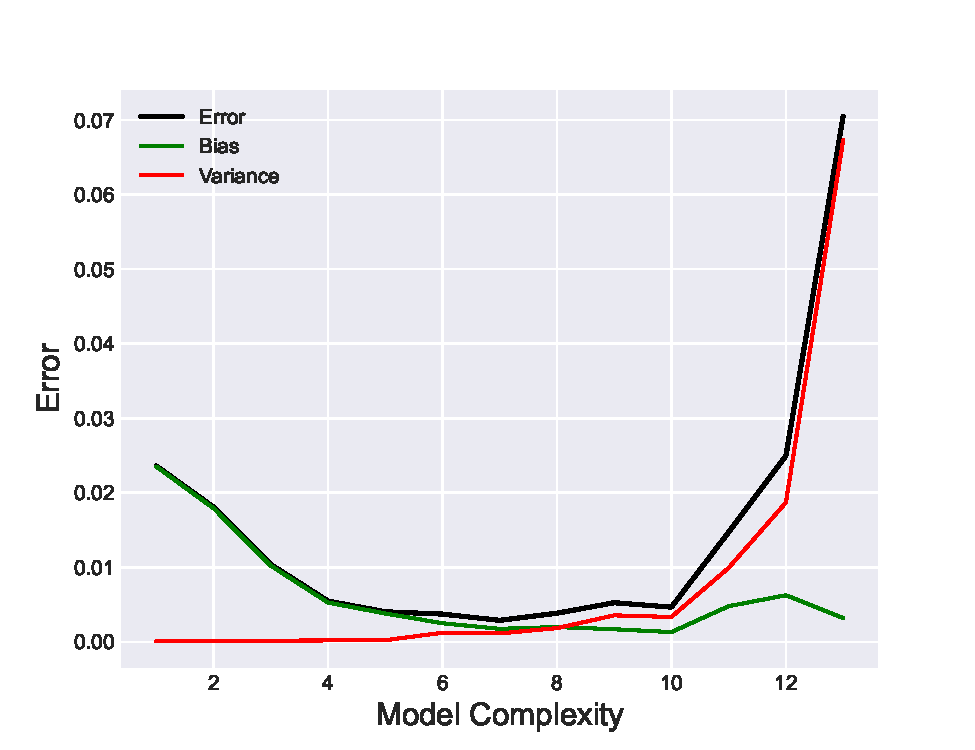
\includegraphics[width=1.1\linewidth]{Bonus task/bonus_fig/biasvar_ols.pdf} 
    \caption{Bias-variance using the OLS method for $n=100$ bootstraps. The complexity is the polynomial degree, shown up to an order of 15.}
    \label{fig: OLS}
\end{figure}
\vspace{3mm}
\\
The data set we approximate is non-linear, and therefore we use linear regression with polynomial features to approximate it. It is thus as expected that a polynomial with degree 1 is insufficient to fit the training samples, as can be seen from the high bias observed for this degree. When using the OLS method, a polynomial of degree 7 obtains a low bias-variance and should therefore approximate the true function much better. For higher degrees the model will overfit the training data, as can be seen from how the variance increases rapidly after a polynomial of degree 10. 
\vspace{3mm}
\\
\begin{figure}[h!]
    \centering %Centers the figure
    \includegraphics[width=1.0\linewidth]{Bonus task/biasvar_ridge2_higher.pdf} 
    \caption{Bias-variance using the Ridge method with $\lambda=1\times 10^{-4}$ (top) and $\lambda=1\times 10^{-9}$ (bottom) for $n=100$ bootstraps. The complexity is the polynomial degree, shown up to an order of 25. Note how a low $\lamda$ parameter makes the model less robust to overfitting.}
    \label{fig: ridge}
\end{figure}
For Ridge, the variance increases only moderately compared to OLS. 
The ridge model is better at handling the error caused by the variance, due to the introduction of the l2 parameter which deals with overfitting. This ensures that the model does not blow up for higher complexity. 
In figure~\ref{fig: ridge} we have visualized two instances for two different l2 parameters. In the lower plot, where $\lambda$ is lower, we can see how the variance increases more, and we get a model closer to the OLS. If we set $\lambda=0$ we would get OLS. For a higher $\lambda$, Ridge achieves a very good model for higher polynomial orders, and overfitting does not seem to become an issue. 
% The lasso model is not as sensitive to low values for $\lambda$, as it uses a hyperparameter $\lambda$ and not $\lambda^2$, like the Ridge method does. Therefore, we should see less overfitting for this model. 

\subsection*{Deep Learning} %_______________________________________________________________________________________
Next, we study the bias-variance for deep learning methods using a Multi-Layer Perceptron (MLP) model. The bias-variance is presented as a function of the number of nodes in one hidden layer in figure~\ref{fig: MLP}. 
As expected, the bias decreases with increasing complexity, before eventually the variance increases. Around 25 neurons, the variance is greater than the bias. It is interesting to see that the lowest error we achieve is greater than what we achieved for both OLS and Ridge. 
\begin{figure}[h!]
    \centering %Centers the figure
    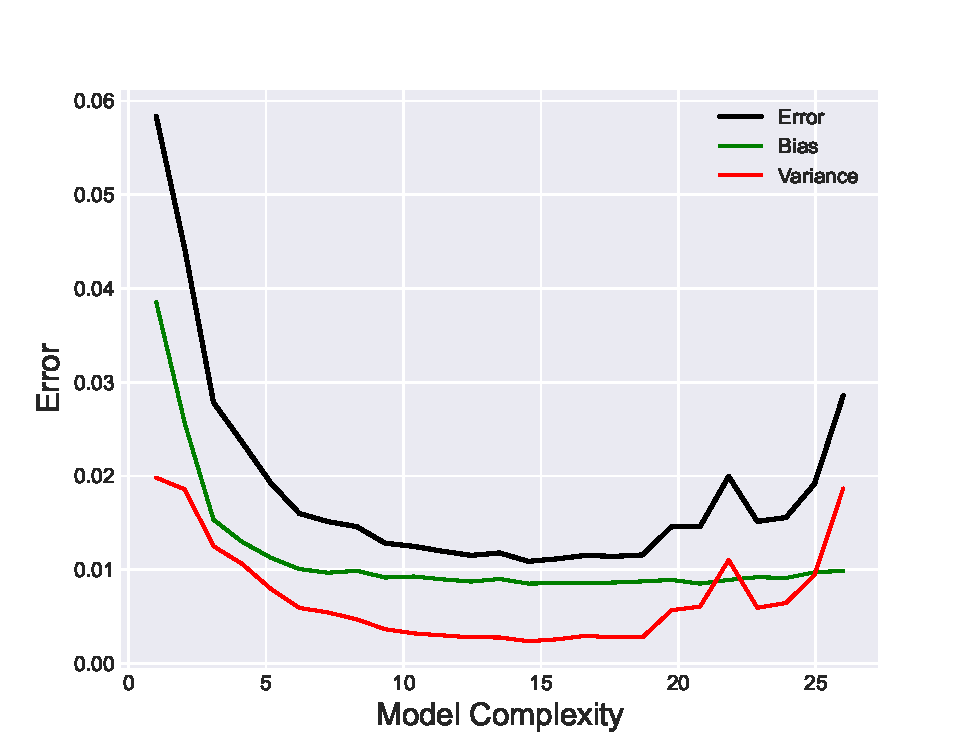
\includegraphics[width=1.1\linewidth]{Bonus task/bonus_fig/biasvar_mlp_one_layer.pdf} 
    \caption{Bias-variance using the FFNN method for a Multi-layer Perceptron regressor for 25 neurons and 1 hidden layer. The number of bootstraps is $n=100$.}
    \label{fig: MLP}
\end{figure}
\vspace{3mm}
\\ 
\begin{figure}[h!]
    \centering %Centers the figure
    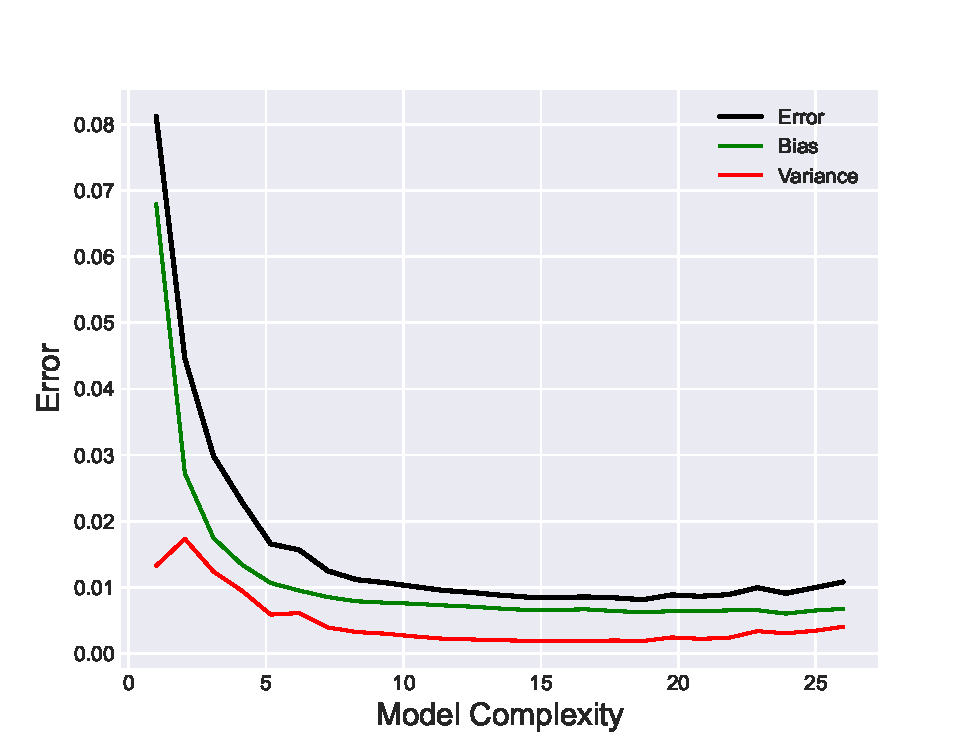
\includegraphics[width=1.1\linewidth]{Bonus task/bonus_fig/biasvar_mlp_two_layers.pdf} 
    \caption{Bias-variance using the FFNN method for a Multi-layer Perceptron regressor for 25 neurons and 2 hidden layers. The number of bootstraps is $n=100$.}
    \label{fig: MLP_two}
\end{figure}
If we increase the number of hidden layers from one to two, we get the plot presented in figure~\ref{fig: MLP_two}. Here, the variance only increases moderately, and the lowest error is somewhat lower than the model with only one layer. While the bias is high in the beginning, it decreases quickly. 
From Neural Network models we expect to see that overfitting becomes more prominent as we increase the complexity~\cite{friedman}, and the variance does begin to increase somewhat as the complexity increases, however not nearly as much as we saw for OLS. 


\subsection*{Ensemble Methods}
Finally, we study two ensemble methods: the decision tree algorithm and the random forests algorithm. 
\vspace{3mm}
\\
Figure~\ref{fig: decisiontree} shows the bias-variance and MSE for a decision tree algorithm trained on the Franke data with a number of bootstraps $n=100$. The complexity corresponds to the maximum depth of the tree
% individual regression estimators
, which limits the number of nodes in the tree~\cite{scikit}. Deeper trees have more complex decision rules and a more complex fitter of the model. As expected, the bias is high for low complexity whilst the variance increases with higher complexity. More complex models generally have a lower bias but a higher variance, and we can see that the variance begins to increase for quite a low order of complexity. 
\begin{figure}[h!]
    \centering %Centers the figure
    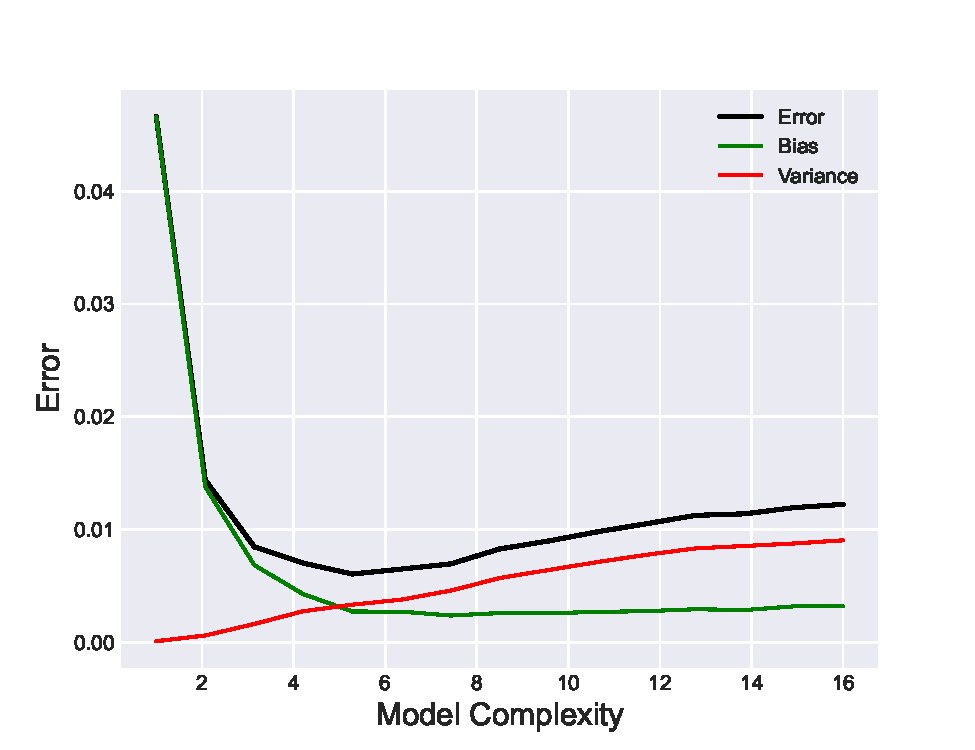
\includegraphics[width=1.1\linewidth]{Bonus task/bonus_fig/biasvar_decisiontrees.pdf} 
    \caption{Bias-variance using the decision tree algorithm on the Franke data set for $n=100$ bootstraps.}
    \label{fig: decisiontree}
\end{figure}
\vspace{3mm}
\\
The basic decision tree method can be used to build more complex networks, such as random forests. In figure~\ref{fig: random} we plot the bias-variance and MSE for such a random forest algorithm trained on the Franke data with a number of bootstraps $n=100$. The bias does not change much from what we saw in figure~\ref{fig: decisiontree}, but the variance is lower, and there is clear improvement in the MSE. This method uses averaging to improve the predictive accuracy and control overfitting, which is the reason for the lower variance even as the complexity is increasing. This allows us to use a more complex model when this is needed. The random forest model therefore remains stable for higher levels of complexity compared to the basic decision tree method. 
\begin{figure}[h!]
    \centering %Centers the figure
    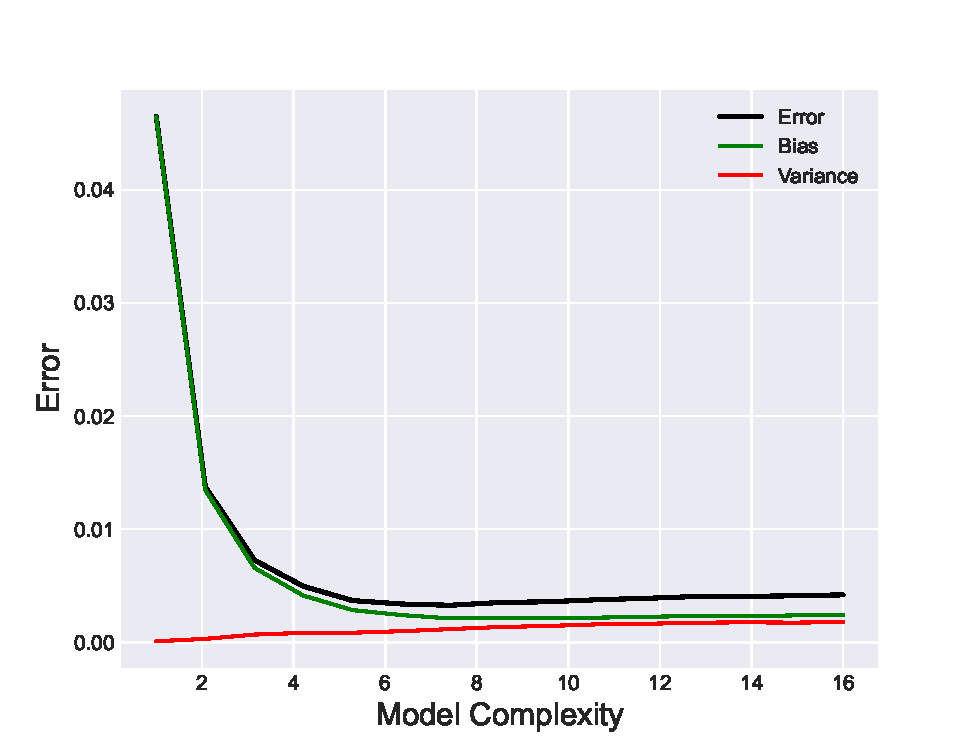
\includegraphics[width=1.1\linewidth]{Bonus task/bonus_fig/biasvar_randomforests.pdf} 
    \caption{Bias-variance using the random forests algorithm on the Franke data set for $n=100$ bootstraps.}
    \label{fig: random}
\end{figure}


\section{Conclusion}\label{sec: conclusion}
Based on our results we have been able to see how the bias and variance vary for different algorithms. Generally, the bias starts off high, before decreasing with increasing complexity, whilst the variance starts of low and will increase with the complexity. This behaviour leads to a point where the MSE is at its lowest, and where we are most likely to avoid both overfitting and underfitting. 
\vspace{3mm}
\\
For OLS the variance quickly became large enough that overfitting was an issue, something that was not observed for the penalized Ridge model. 
Overfitting generally was not an issue for Ridge, MLP or random trees. Ridge and random trees behave in a similar manner, with the variance increasing slowly for higher complexity, but the bias decreases more quickly for the random trees method. Both achieve a low error, but Ridge unexpectedly achieves the lowest of the two. Ridge is also more computationally efficient, and so it seems as if this model is a better choice, based on computational time and performance. 
\vspace{3mm}
\\ 
Generally, when choosing the best model and parameters for a data set, we have to consider the type of data set.
The linear regression methods we study are well suited for lower complexity models, as they often require less computational time. However, many models require more complexity and flexibility, making random forests, or other variations of decision trees good choices. 
In this case, it seems that that Ridge is the optimal models in terms of bias-variance, error, and computational time. While all methods are able to obtain a low bias-variance, Ridge manages to do so consistently, for higher levels of complexity. 

\bibliography{sources}
\end{document}